With the leading order and next-to-leading order \chpt, Lagrangian, we can now compute thermodynamic properties such as the free energy and the equation of state and investigate the phase transition to the pion condensate phase.
We will start with the free energy, computing the leading-order contribution to one loop, and the next-to-leading order contribution at tree-level, following the procedure used in~\autocite{adhikariTwoflavorChiralPerturbation2019,martinariaTwoflavorChiralPerturbation2020}.\footnote{Leading order and next-to-leading order, in this context, refers to Weinberg's power counting scheme.}



\section{*Free energy at lowest order}
\label{section: free energy at lowest order}
\todo[inline]{combine with pion star chapter}

The free energy density of a homogenous system is
%
\begin{equation}
    \Eff = - \frac{1}{V \beta} \ln \mathcal{Z}.
\end{equation}
%
Here, $\mathcal{Z}$ is the partition function, $V$ is the volume of space, and $\beta = 1/T$ is inverse temperature.
Using imaginary-time formalism for thermal field theory, described in \autoref{appendix: thermal field theory}, we find that the partition function is given by the path integral of the \emph{Euclidean} Lagrange density, as shown in equation \autoref{free scalar result 2}.
In the zero temperature limit  $\beta \rightarrow \infty$, the partition function is related to the generating functional $Z = Z[j]$, as described in \autoref{section: path integral}, by a Wick rotation.
The free energy density at zero temperature is therefore
%
\begin{equation}
    \Eff = \frac{i}{VT} \ln Z,
\end{equation}
%
where $VT$ is the volume of space-time.
This equals the effective potential in the ground state.
In \autoref{section: effective action}, we found an explicit formula for this to one-loop order, \autoref{effective potential}.
We write $\Eff = \Eff^{(0)} + \Eff^{(1)} + \dots$, where $\Eff^{(n)}$ refers to the $n$-loop contributions to the free energy density.


\subsection{Tree-level contribution}

The tree-level contribution $\Eff^{(0)}$ is the classical potential, which is given by the static ($\pi$-independent) part of the Lagrangian.
From \autoref{L0} we have the leading order contribution,
%
\begin{equation}
    \label{leading order contribution free energy}
    \Eff_2^{(0)}
    = - \Ell_2^{(0)} 
    = 
    -f^2   
    \left(
        \bar m^2 \cos{\alpha}
        + \frac{1}{2} \mu_I^2 \sin^2{\alpha}
    \right),
\end{equation}
%
where $\alpha$ parameterizes the ground state.
This parameter must minimize the free energy, which means that
%
\begin{align}
    &\pdv{}{\alpha} \Eff_2^{(0)} 
    = f^2\left(\bar m^2 - \mu_I^2\cos{\alpha}\right)\sin{\alpha}
    = 0.
\end{align}
%
This equation defines the relationship between the chemical potential $\mu_I$ and $\alpha$, as illustrated in \autoref{fig: free energy surface}.
This gives the criterion
%
\begin{align}
    \label{leading order minimization}
    \alpha \in \{0, \pi\} \quad
    \mathrm{or} \quad
    \cos{\alpha} = \frac{\bar m^2}{\mu_I{}^2}.
\end{align}
%
As we see in the figure, $\alpha = \pi$ is a maximum and thus unstable.
This means that for all values $\mu_I^2 \leq \bar m^2$, we will have $\alpha = 0$, and the system will remain in the vacuum.

In our discussion of the effective potential, we also found that the ground state should minimize the classical potential, as shown by \autoref{minimize classical potential}.
As a consequence, the linear part of the classical potential should vanish.
The linear part of the classical potential is given by \autoref{L1} to leading order. It reads $\Ve^{(1)} = f(\mu_I{}^2\cos{\alpha} - \bar m^2)\sin{\alpha} \, \pi_1 $, and vanishes given the minimizition criterion \autoref{leading order minimization}.
\todo[]{include figure}
\begin{figure}[ht]
    \centering
    % 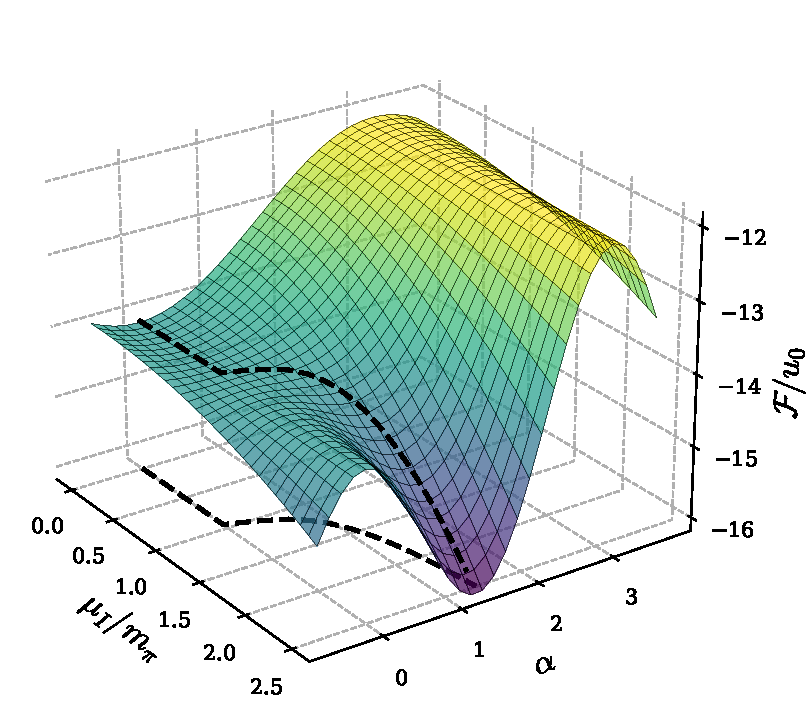
\includegraphics{../scripts/numerikk/plots//free_energy_surface.pdf}
    \caption{
        The free energy surface as a function of $\mu_I$ and $\alpha$. $\alpha$ is the found by minimizing $\Eff$ for a given $\mu_I$. This leads to a curve across the free energy surface, as show in the plot.
        }
    \label{fig: free energy surface}
\end{figure}



\subsection{One-loop contribution}

The one-loop contribution to the free energy density is
%
\begin{equation}
    \label{one loop free energy}
    \Eff^{(1)}
    = - \frac{i}{V T} \frac{1}{2}
    \Tr{\ln\left( -\fdv{S[\pi = 0]}{\pi_a(x), \pi_b(y)} \right)}.
\end{equation}
%
This can be evaluated using the rules for functional differentiation given in \autoref{appendix: Functional derivatives}.
To leading order,
%
\begin{align}
    \fdv{S[\pi = 0]}{\pi_a(x), \pi_b(y)}
    = \fdv{}{\pi_a(x), \pi_b(y)}
    \int \dd^4 x \, \Ell^{(2)}_2
    = D_{ab}^{-1}(x - y).
\end{align}
%
Here, $\Ell^{(2)}_2$ is the quadratic part of the Lagrangian, as given in \autoref{quadratic lagrangian}, and $D^{-1}$ is the corresponding inverse propagator of the pion fields,
\begin{equation}
    D_{ab}^{-1}(x-y) = 
    \left[
        - \delta_{ab}(\partial_x^2 + m^2_a)
        + m_{12}(\delta_{a1} \delta_{b2} - \delta_{a2}\delta_{b1}) \partial_{x, 0}
    \right] \delta(x-y)
\end{equation}
%
The inverse propagator is a matrix, which means that the determinant in \autoref{one loop free energy} is both a matrix determinant, over the three pion indices, and a functional determinant.
In \autoref{section: propagator} we found the matrix part of the determinant in momentum space, which we can write using the dispersion relations of the pion fields
\begin{equation}
    \det(- D^{-1}) = \det(-p_0^2 + E_0^2) \det(-p_0^2 + E_+^2) \det(-p_0^2 + E_-^2).
\end{equation}
%
These dispersion relations are functions of the three-momentum $\vec p$, and are given in \autoref{dispresion relation pi 0} and \autoref{dispresion relation pi pm}.
The functional determinant can therefore be evaluated as
%
\begin{align}
    \nonumber
    \Tr{\ln\left( -\fdv{S[\pi = 0]}{\pi_a(x), \pi_b(y)} \right)}
    & = \ln \det(-p_0^2 + E_0^2) + \ln \det(-p_0^2 + E_+^2) + \ln \det(-p_0^2 + E_-^2) \\
    \nonumber
    & = \Tr{ \ln(-p_0^2 + E_0^2) + \ln(-p_0^2 + E_+^2)+  \ln(-p_0^2 + E_-^2) } \\
    & = (VT) \int \frac{\dd^4 p}{(2 \pi)^4} 
    \left[ \ln(-p_0^2 + E_0^2) + \ln(-p_0^2 + E_+^2) + \ln(-p_0^2 + E_-^2)  \right],
\end{align}
%
where we have used the identity $\ln\det M = \Tr \ln M $.
These terms all have the form
%
\begin{equation}
    \label{free energy logarithmic integral}
    I = \int \frac{\dd^4 p}{(2 \pi)^2} \ln(-p_0^2 + E^2),
\end{equation}
%
where $E$ is some function of the 3-momentum $\vec p$, but not $p_0$.
We use the trick
%
\begin{equation}
    \pdv{}{\alpha} \left(-p_0^2 + E^2\right)^{-\alpha} \Big|_{\alpha=0}
    = \pdv{}{\alpha} \exp {-\alpha \ln\left(- p_0^2 + E^2\right)} \Big|_{\alpha=0}
    = \ln\left(- p_0^2 + E^2\right),
\end{equation}
%
and then perform a Wick-rotation of the $p_0$-integral to write the integral on the form 
%
\begin{equation}
    I = i \pdv{}{\alpha} \int \frac{\dd^4 p}{(2 \pi)^4} \left(p_0^2 + E^2\right)^{-\alpha} \Big|_{\alpha=0},
\end{equation}
%
where $p$ now is a Euclidean four-vector.
The $p_0$ integral equals $\Phi_1(E, 1, \alpha)$, as defined in \autoref{def dimreg integral}. 
The result is therefore given by \autoref{result dimreg},
%
\begin{equation}
    \int \frac{\dd p_0}{2 \pi} (p_0^2 + E)^{-\alpha} 
    = \frac{E^{1-2\alpha}}{\sqrt{4 \pi}} \frac{\Gamma(\alpha-\frac{1}{2})}{\Gamma(\alpha)}.
\end{equation}
%
The derivative of the Gamma function is $\Gamma'(\alpha) = \psi(\alpha)\Gamma(\alpha)$, where $\psi(\alpha)$ is the digamma function.
Using
%
\begin{align}
    \pdv{}{\alpha} & \frac{\Gamma(\alpha - \frac{1}{2}) }{\Gamma(\alpha)} \Big|_{\alpha=0}
    = \Gamma\left(\alpha - \frac{1}{2}\right) \frac{\psi(\alpha - \frac{1}{2}) - \psi(\alpha)}{\Gamma(\alpha)} \Big|_{\alpha=0}
    = \sqrt{4 \pi}, \\
    & \frac{\Gamma(\alpha - \frac{1}{2}) }{\Gamma(\alpha)}\Big|_{\alpha=0} = 0,
\end{align}
%
we get
%
\begin{equation}
    I = i \int \frac{\dd^3 p}{(2 \pi)^3} E.
\end{equation}
%
We see that the result is what we would expect physically; the total energy is the integral of each mode's energy.
This also agrees with the result from \autoref{appendix: thermal field theory} in the zero-temperature limit $\beta \rightarrow \infty$.
The one-loop contribution can therefore be written
%
\begin{equation}
    \Eff^{(1)} = 
    \frac{1}{2} 
    \left[\int \frac{\dd^3 p}{(2\pi)^3} E_0 + \int  \frac{\dd^3 p}{(2\pi)^3} (E_+ + E_-)\right]
    = \Eff^{(1)}_{\pi_0} +\Eff^{(1)}_{\pi_\pm}.
\end{equation}
%
The first integral is identical to what we find for a free field in \autoref{section:free scalar field}, in the zero-temperature limit.
These terms are all divergent and must be regularized.
We will use dimensional regularization, in which the integral is generalized to $d$ dimensions, and the $\overline{\mathrm{MS}}$-scheme, as described in \autoref{section: regualting free energy}.
Using the result for a free field \autoref{free field regularized energy}, we get
%
\begin{equation}
    \label{Free energy pi 0}
    \Eff^{(1)}_{\pi_0} 
    = 
    - \mu^{-2 \epsilon}  \frac{1}{4} \frac{m_3^4}{(4\pi)^2} 
    \left( \frac{1}{\epsilon} + \frac{3}{2} + \ln \frac{\tilde \mu^2}{m_3^2} \right)
    + \mathcal{O}(\epsilon),
\end{equation}
%
where $\mu$ is the renormalization scale, a parameter with mass-dimension 1, introduced to ensure the action integral remains dimensionless during dimensional regularization.
$\tilde \mu$ is a related to $\mu$ as described in \autoref{definition mu tilde MS bar}.

The contribution to the free energy from the $\pi_+$ and $\pi_-$ particles is more complicated, as the dispersion relation is given by
%
\begin{equation}
    E_\pm
    = 
    \sqrt{
        |\vv p|^2 +
        \frac{1}{2}
        \left(
            m_1^2 + m_2^2 + m_{12}^2 
        \right)
        \pm 
        \frac{1}{2}
        \sqrt{
            4|\vv p|^2m_{12}^2 
            +
            \left(
                m_1^2 + m_2^2 + m_{12}^2
            \right)^2
            - 4 m_1^2 m_2^2
        }
    }.
\end{equation}
%
This is not an integral we can easily do in dimensional regularization.
Instead, we will seek a function $f(|\vv p|)$ with the same UV-behavior, that is, behavior for large $\vv p$, as $E_+ + E_-$.
If we then add $0 = f(|\vv p|) - f(|\vv p|)$ to the integrand, we can isolate the divergent behavior
%
\begin{equation}
    \Eff_{\pi_\pm}^{(1)}
    = 
    \frac{1}{2} \int \frac{\dd^3 p}{(2\pi)^3} [E_+ + E_- + f(|\vv p|) - f(|\vv p|)]
    = \Eff^{(1)}_{\mathrm{fin}, \pi_\pm } + \Eff^{(1)}_{\mathrm{div}, \pi_\pm}.
\end{equation}
%
This results in a finite integral,
%
\begin{equation}
    \Eff^{(1)}_{\mathrm{fin}, \pi_\pm } = \frac{1}{2} \int \frac{\dd^3 p}{(2\pi)^3} [E_+ + E_- - f(|\vv p|)],
\end{equation}
%
which we can evaluate numerically, and a divergent integral
%
\begin{equation}
    \Eff^{(1)}_{\mathrm{div}, \pi_\pm }
    = 
    \frac{1}{2} \int \frac{\dd^3 p}{(2\pi)^3} f(|\vv p|),
\end{equation}
%
which we hopefully will be able to do in dimensional regularization.
We can explore the UV-behavior of $E_+ + E_-$ by expanding it in powers of $1 / \abs{\vv{p}}$,
%
\begin{align}
    \nonumber
    E_+ + E_-
    & = 
    2  \abs{\vv{p}}
    + \frac{m_{12} + 2(m_1^2 + m_2^2)}{4} \, {\abs{\vv{p}}}^{-1}
    - \frac{m_{12}^4 + 4 m_{12}^2(m_1^2 + m_2^2) + 8(m_1^4 + m_2^4)}{64}
    {\abs{\vv{p}}}^{-3}
    + \Oh (\abs{\vv{p}}^{-5})
    \\
    & = 
    a_1  \abs{\vv{p}}
    + a_2 \, {\abs{\vv{p}}}^{-1}
    + a_3
    {\abs{\vv{p}}}^{-3}
    + \Oh (\abs{\vv{p}}^{-5}).
\end{align}
%
We have defined new constants $a_i$ for brevity of notation.
As
%
\begin{equation}
    \int_{\R^3} \frac{\dd^3 p}{(2 \pi)^3} |\vv p|^{n}
    = C \int_{0}^\infty \dd p \, p^{2 + n}
\end{equation}
%
is UV divergent for $n \geq -3$, $f$ need to match the expansion of $E_+ + E_-$ up to and including $\Oh(|\vv{p}|^{-3})$ for $\Eff^{(1)}_{\mathrm{fin}, \pi_\pm }$ to be finite.
The most obvious choice for $f$ is
%
\begin{equation}
    f(|\vv p|) 
    = a_1  \abs{\vv{p}} + a_2 \, {\abs{\vv{p}}}^{-1} + a_3 \, {\abs{\vv{p}}}^{-3}.
\end{equation}
%
However, this introduces a new problem.
$f$ has the same UV-behavior as $E_+ + E_-$, but the last term diverges in the IR, that is, for low $|\vv p|$.
This can be amended by introducing a mass term.
Let
%
\begin{equation}
    |\vv p|^{-3} 
    = 
    \left(\frac{1}{\sqrt{|\vv p|^2}}\right)^3 
    \longrightarrow 
    \left(\frac{1}{\sqrt{|\vv p|^2 + m^2}}\right)^3.
\end{equation}
%
For $|\vv p|^2 \rightarrow \infty$, this is asymptotic to $|\vv p|^{-3}$, so it retains its UV behavior.
However, for $|\vv p| \rightarrow 0$, it now approaches $m^{-3}$, so the IR-divergence is gone.
The cost of this technique is that we have introduced an arbitrary mass parameter.
Any final result must thus be independent of the value of $m$ to be acceptable.

We will instead regularize the integral by defining $E_i = \sqrt{|\vv{p}|^2 + \tilde m_i^2}$, and $\tilde m_i^2 = m_i^2 + \frac{1}{4} m_{12}^2$.
Using the definition of the masses, \autoref{m1}, \autoref{m2}, \autoref{m3}, and \autoref{m12}, we get
%
\begin{align}
    m_3^2 & = \bar m^2 \cos \alpha + \mu_ I^2 \sin^2 \alpha, \\
    \label{tilde m1}
    \tilde m_1^2 
    & 
    = m_1^2 + \mu^2 \cos\alpha^2
    = \bar m^2 \cos \alpha + \mu_I^2 \sin^2 \alpha
    = m_3^2 \\
    \label{tilde m2}
    \tilde m_2^2 
    & = m_2^2 + \mu^2 \cos\alpha^2
    = \bar m^2 \cos \alpha.
\end{align}
%
Finally, we define $f(|\vv p|) = E_1 + E_2$, which differ from $E_+ + E_-$ by $\Oh\left(|\vv p|^{-5}\right)$ and is well-behaved in the IR.
This leads to a divergent integral the same form as in the case of a free scalar.
Thus, in the $\mathrm{\overline{MS}}$-scheme, 
%
\begin{equation}
    \Eff^{(1)}_{\mathrm{div}, \pi_\pm }
    =
    - \mu^{-2 \epsilon} \frac{1}{4} \frac{\tilde m_1^4}{(4\pi)^2} 
    \left(
        \frac{1}{\epsilon} + \frac{3}{2} + \ln \frac{\tilde \mu^2}{\tilde m_1^2}
    \right) 
    -  \mu^{-2 \epsilon} \frac{1}{4} \frac{\tilde m_2^4}{(4\pi)^2} 
    \left(
        \frac{1}{\epsilon} + \frac{3}{2} + \ln \frac{\tilde \mu^2}{\tilde m_2^2}
    \right) 
    + \mathcal{O}(\epsilon).
\end{equation}
%
We define
%
\begin{equation}
    \Eff^{(1)}_{\mathrm{fin}, \pi_\pm}
    = 
    \frac{1}{2} \int \frac{\dd^3 p}{(2\pi)^3} (E_+ + E_- - E_1 - E_2),
\end{equation}
%
which is a finite integral.
The total one-loop contribution is then, using \autoref{tilde m1} and \autoref{tilde m2},
%
\begin{align}
    \Eff^{(2)}
    & = 
    \Eff^{(1)}_{\mathrm{fin}, \pi_\pm}
    - \mu^{-2 \epsilon} \frac{1}{2}\frac{1}{(4\pi)^2}
    \left[
        \left( \frac{1}{\epsilon} + \frac{3}{2} + \ln \frac{\tilde \mu^2}{m_3^2 } \right)
        m_3^4
        +
        \frac{1}{2}
        \left( \frac{1}{\epsilon} + \frac{3}{2} + \ln \frac{\tilde \mu^2}{\tilde m_2^2} \right)
        \tilde m_2^4
    \right]
    + \Oh(\epsilon).
\end{align}

